\documentclass{standalone}
\usepackage{tikz}
\usepackage{tikz-qtree}
\usepackage{xcolor}
\usetikzlibrary{arrows}
\usepackage{fontspec}
\setmainfont{Helvetica}
\begin{document}
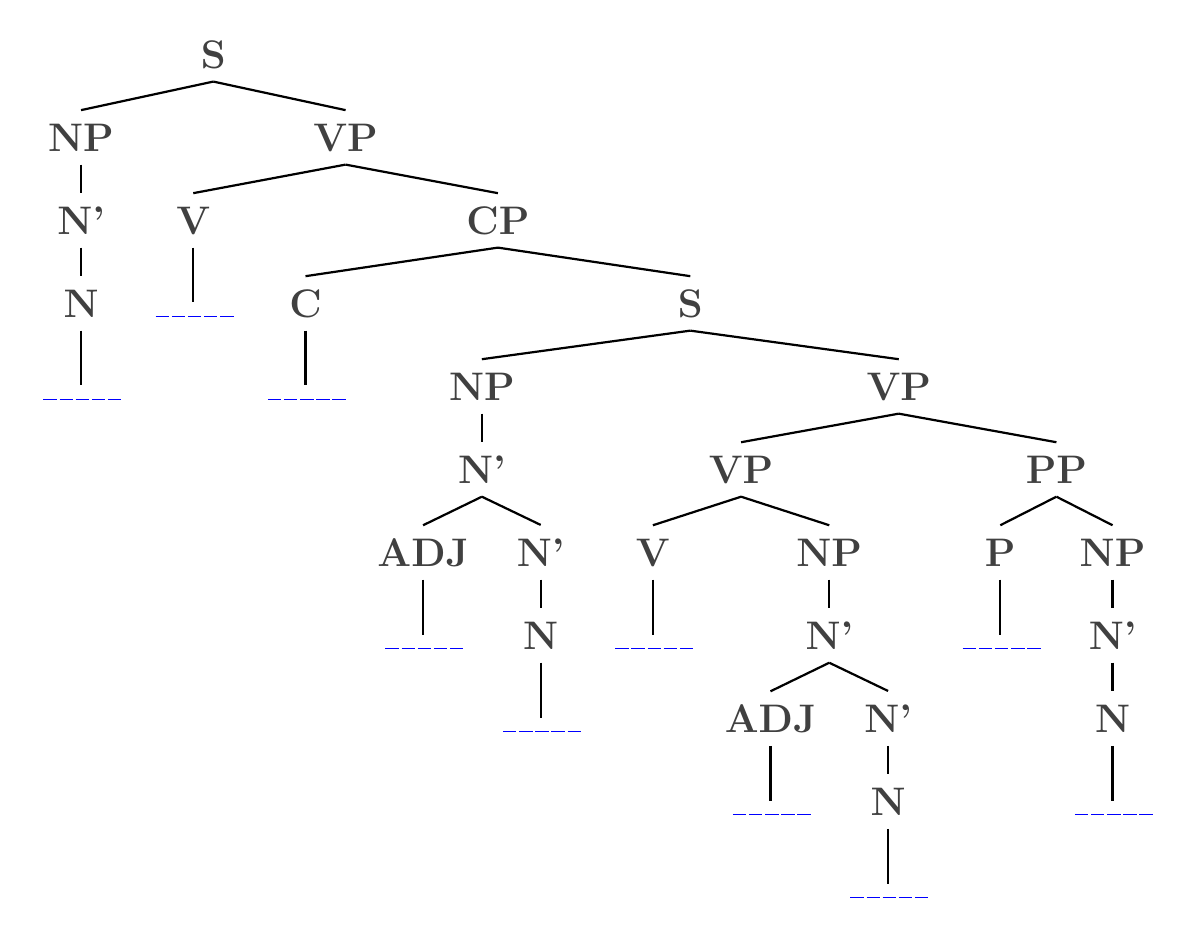
\begin{tikzpicture}
\tikzset{level distance=30pt}
\tikzset{every  leaf node/.style={text=blue,font=\bf}}
\tikzset{every internal node/.style={text=darkgray,font=\bf}}
\tikzset{edge from parent/.append style={thick}}

\Large

\Tree[.S [.NP [.N' [.N \_\_\_\_\_ ] ] ] [.VP [.V \_\_\_\_\_ ] [.CP [.C \_\_\_\_\_ ] [.S [.NP [.N' [.ADJ \_\_\_\_\_ ] [.N' [.N \_\_\_\_\_ ] ] ] ] [.VP [.VP [.V \_\_\_\_\_ ] [.NP [.N' [.ADJ \_\_\_\_\_ ] [.N' [.N \_\_\_\_\_ ] ] ] ] ] [.PP [.P \_\_\_\_\_ ] [.NP [.N' [.N \_\_\_\_\_ ] ] ] ] ] ] ] ] ]


\end{tikzpicture}
\end{document}
